\chapter{CPU-Net Result}\label{chap:cpu-net_result}

\section{Introduction}

Neutrinoless double-beta decay is primarily a single-site event. LEGEND thus seeks to distinguish between single-site and multi-site events using PSD techniques. In order to have accurate simulations, the ATN needs to replicate the correct ensemble distribution for the distribution. The FEP peak is an excellent region for training given that it has a lot of events and it contains a mixture of single and multi-site events. SEP and DEP peaks can then be used as a validation data set, evaluating the model's response to multi-site and single-site events, respectively. We trained the CPU-Net on 110,000 FEP waveforms and then used the SEP and DEP for validation. In this chapter, we present the result analysis of ATN's ability to reproduce detector waveforms using some critical parameters used in PSD. 


\section{Training progression}
The progression of training losses is shown in Figure \ref{fig:training_loss}. The cycle-consistent and identity losses converge rapidly towards zero. The adversarial training is evident in the losses for the discriminators and generators. Early in training, the discriminator initially `wins' and its loss decreases while the generator’s loss increases. As training continues, the generator catches up and the networks approach an equilibrium in which each attempts to out-compete the other. Thus, the loss functions fluctuate as they continuously adapt and improve.


\begin{figure}%[htb!]
    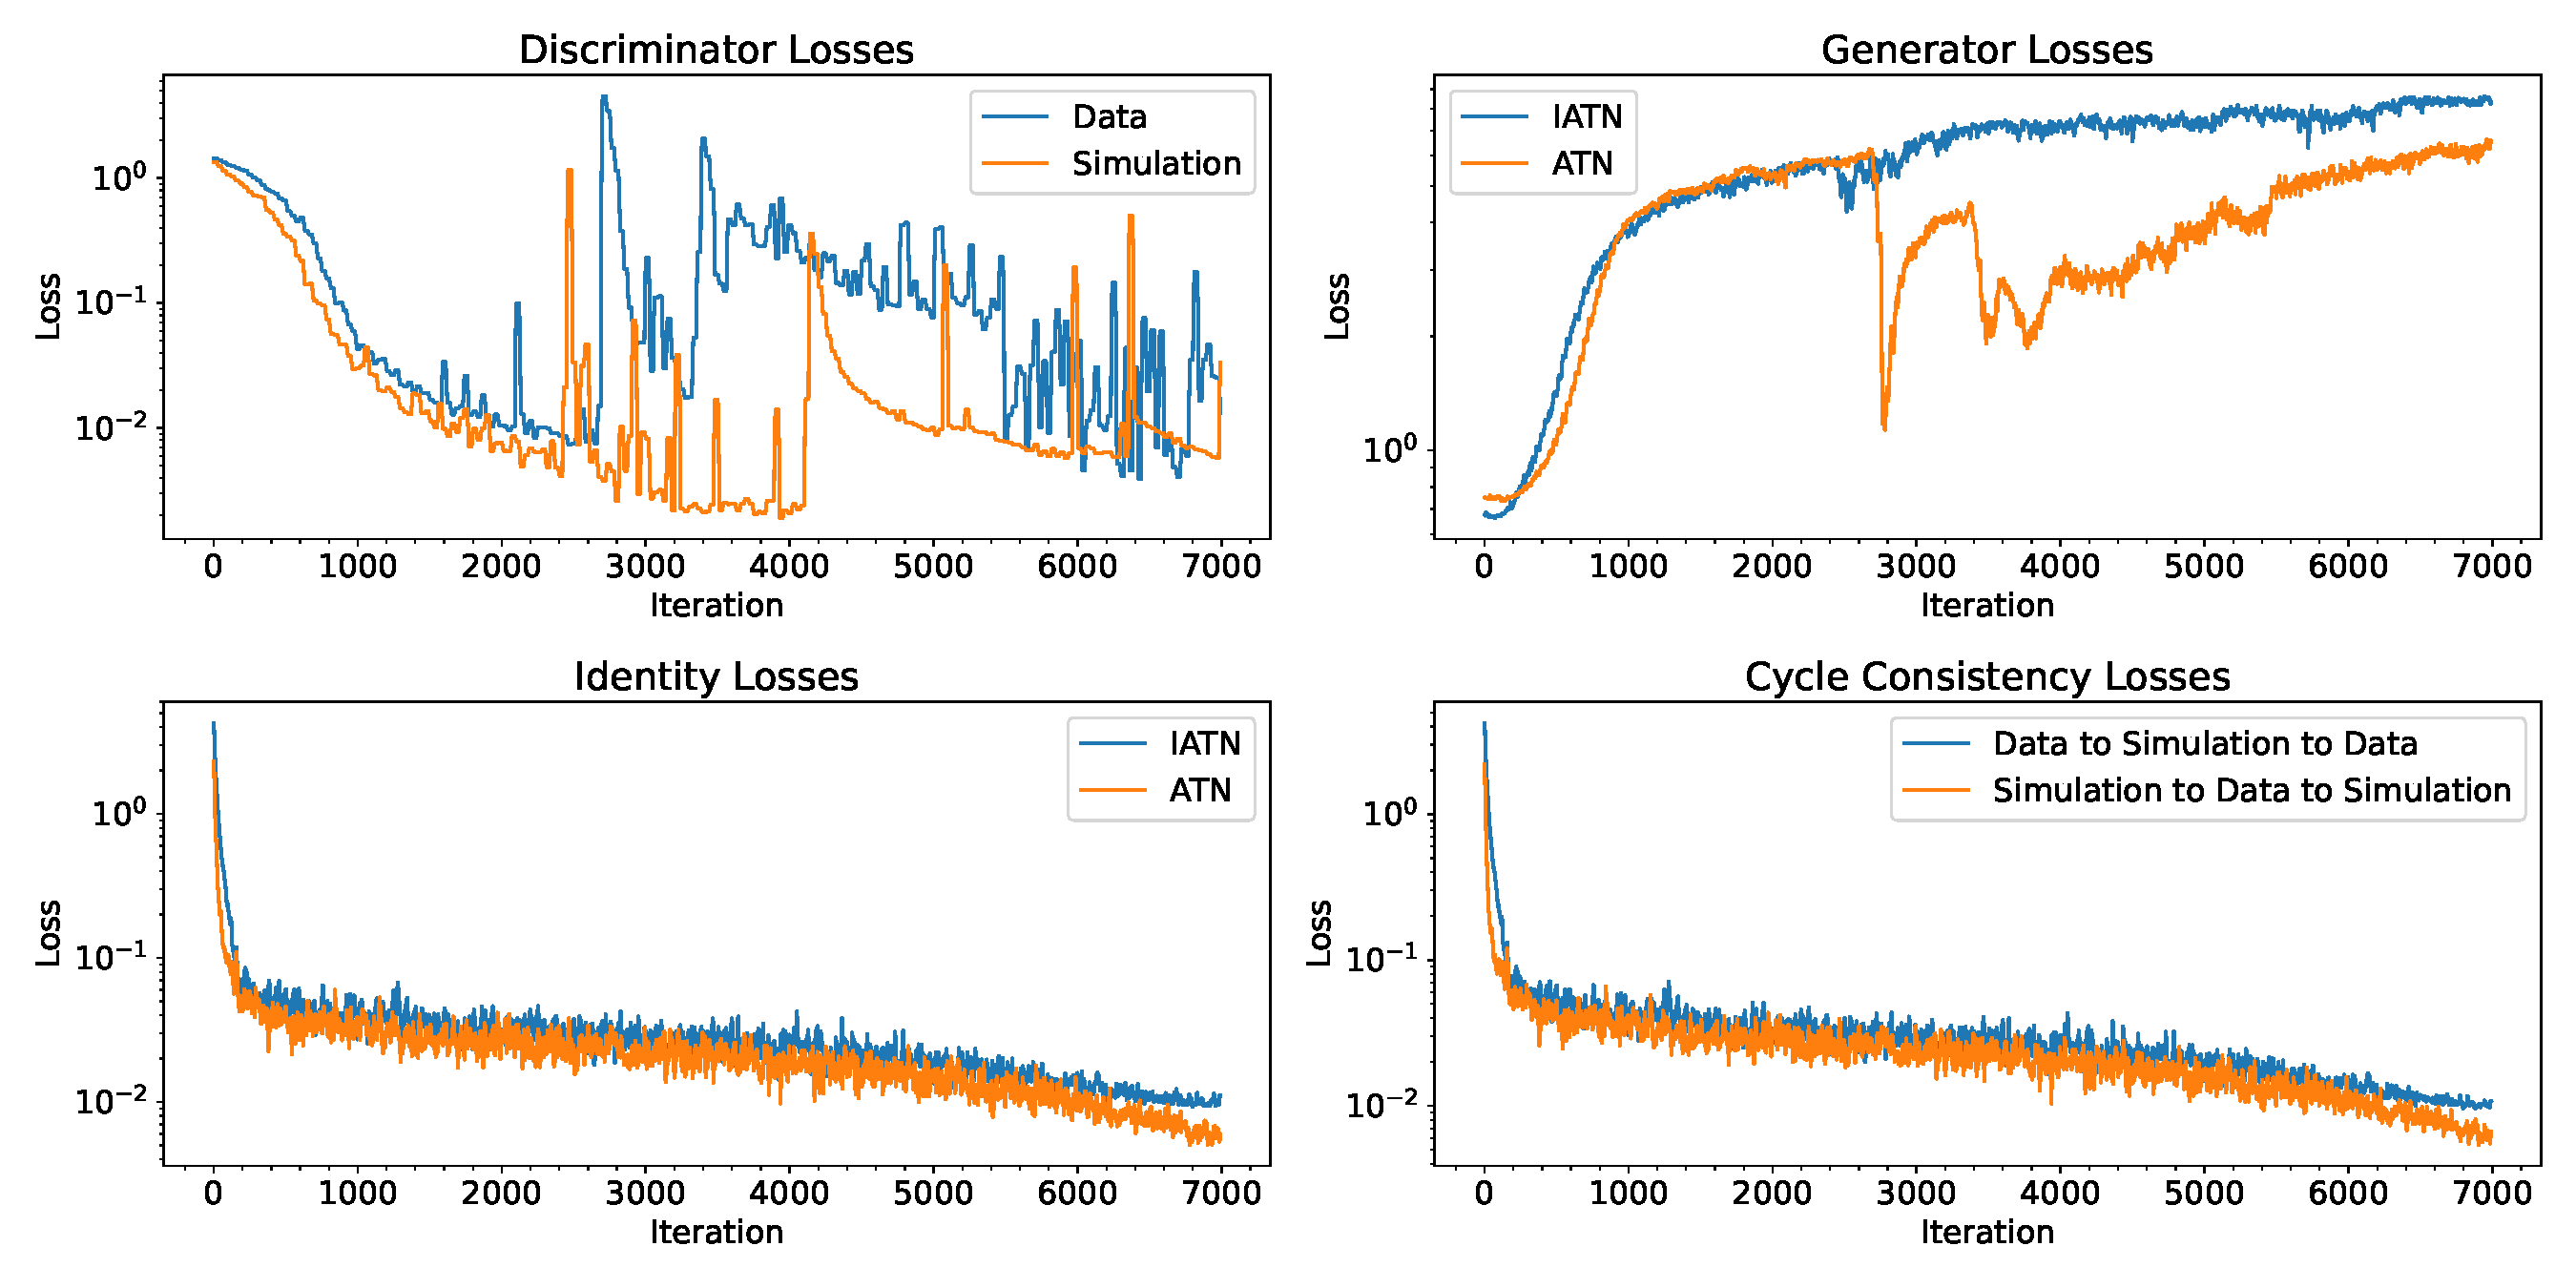
\includegraphics[width=0.99\linewidth]{ch8/figs/loss_funcs.pdf}
    \caption{Training losses for CPU-Net. Losses have been smoothed using a moving average of 10 samples for clarity. The identity and Cycle losses rapidly converged to zero while the generator and discriminator losses fluctuate.} 
   \label{fig:training_loss}
\end{figure}

 % The translation of simulated waveform is shown in Fig \ref{fig:current_amp}. The ATN translates the simulated waveform to the ATN output by smoothing the sharp turning edge in the grey region. This is a consequence of the non-zero integration time in detector waveforms, which is set to $0$ in {\siggen}. The RC discharge effect of the electronic readout system is also set to 0 in {\siggen}, leading to a tail slope of 0 in the simulated waveforms. The ATN learns to translate the flat tail in the cyan region into an exponential decay, and the strength of the decay can be measured by the tail slope reconstruction parameter $c_{tail}$.

% \begin{figure}[htb!]
%     \includegraphics[width=0.99\linewidth]{ch8/figs/ATN.png}
%     \caption{An example ATN output (blue) generated by the input simulated waveform (red). A detector waveform (dotted magenta,randomly drawn from data) is also illustrated as a reference. The grey region depicts the area where the preamplifier integration effect is most visible. The blue region shows the impact of the RC circuit discharge effect.} 
%    \label{fig:sample_result}
% \end{figure}

\section{Waveform Translation}
Figure \ref{fig:cycle_bab} and \ref{fig:cycle_aba} show the cycle consistency in the CPU-Net on the SEP waveforms. The network effectively translates the waveforms in forward and reverse translations. In the {\siggen} simulations, the RC discharge effect is not modeled, resulting in a flat tail slope of zero. ATN learns to transform this flat tail into an exponentially decaying one, matching the observed behavior in real detector data, and IATN learns to transform it back to a zero slope, matching the simulations.

% A simple way to understand the electronics response is to look at the signal waveform tail. . This is usually corrected in post signal processing stage where the `pole' cause by the RC decay is corrected by integrating a `zero' into the transfer functions, called pole-zero correction. While the pole-zero correction has proved reliable for HPGe experiments, it is a first order correction and often higher corrections are warranted. \cite{MJD_electronics}\cite{mjd_pole_zero}

\begin{figure}[htb!]
    \centering
    %trim={0pc 0pc 0pc 3pc},clip
    \includegraphics[width=0.99\linewidth]{ch8/figs/SEP_result_comp_1x3_cycle_BAB.pdf}
    \caption{Illustration of bi-directional cycle consistency in waveform translation in forward direction. Starting with 10 simulated waveforms, the ATN first translates them into detector-like waveforms, and then IATN translates them back to the simulation like waveforms.}
    \label{fig:cycle_bab}
\end{figure}

\begin{figure}[htb!]
    \centering
    %trim={0pc 0pc 0pc 3pc},clip
    \includegraphics[width=0.99\linewidth]{ch8/figs/SEP_result_comp_1x3_cycle_ABA.pdf}
    \caption{Illustration of bi-directional cycle consistency in waveform translation in backward direction. Beginning with 10 detector waveforms, the IATN translates them into simulated-like waveforms, and then ATN translates back to detector-like waveforms.}
    \label{fig:cycle_aba}
\end{figure}

\section{Validation of Key Waveform Parameters}
 The accuracy of translations can be assessed at a distributional level by plotting the histogram of key reconstruction parameters. We use the Intersection over Union (IoU) metric to measure the overlap between distributions.
 
\subsection{Drift Time Distribution}

- how drift time is calculated.


\begin{figure}[!htb]
    \centering
    %trim={0pc 0pc 0pc 3pc},clip
    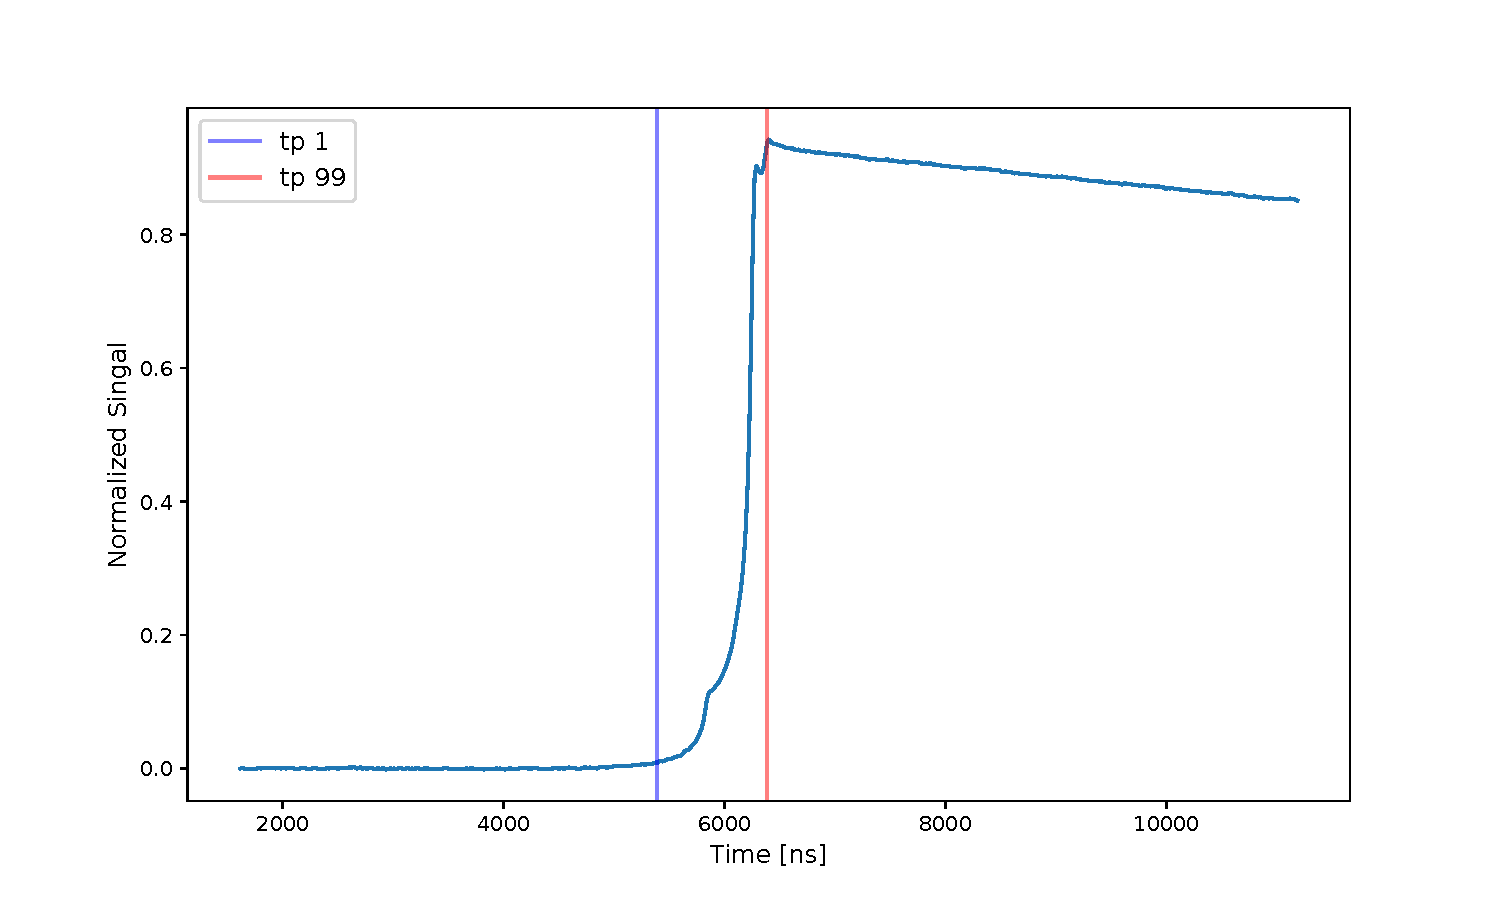
\includegraphics[width=0.99\linewidth]{ch8/figs/time_calc.pdf}
    \caption{Calculating the time points of the waveform}
    \label{fig:ch8:time_calc}
\end{figure}


 Figures \ref{fig:drift_times_sep} and \ref{fig:drift_times_dep} illustrate the distribution of drift time $T_{Drift}$. Data show a slower $T_{Drift}$ due to the influence of the preamplifier. ATN nets learn to slow the drift time of the waveforms while keeping matching the distribution of the data.  The SEP $T_{Drift}$ IoU increases to $62.4\%$ from $39.5\%$.
 
\begin{figure}[!htb]
%[trim={left bottom right top},clip]
\centering
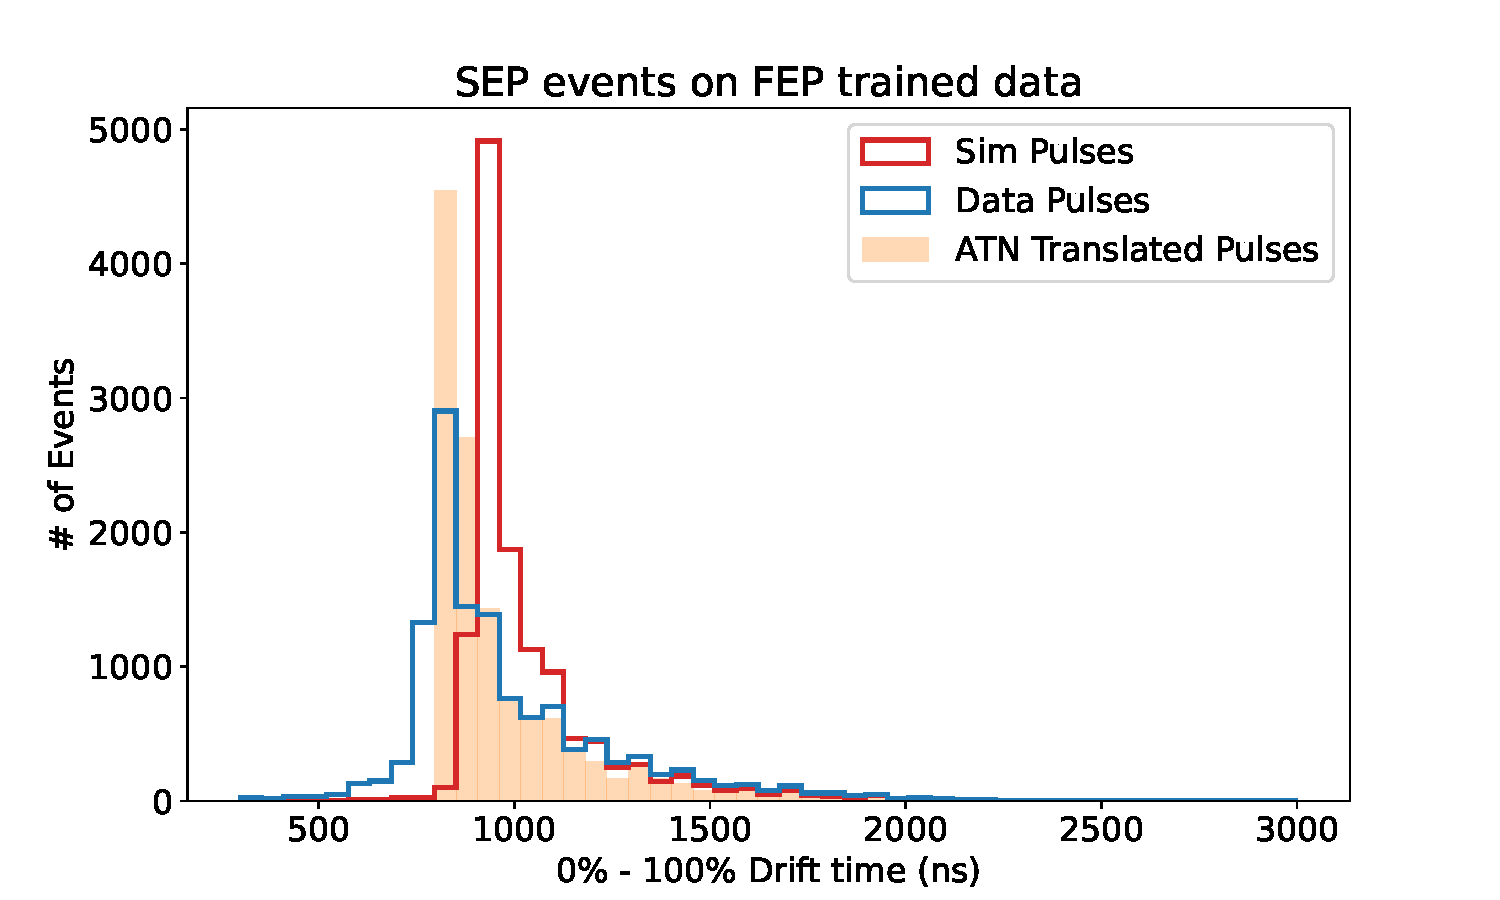
\includegraphics[width=0.99\linewidth,trim={0pc 0pc 0pc 0pc},clip]{ch8/figs/sep_drift_time.pdf}
\caption{The distribution of the 1\%–100\% drift time on SEP dataset.}
\label{fig:drift_times_sep}
\end{figure}

\begin{figure}[!htb]
%[trim={left bottom right top},clip]
\centering
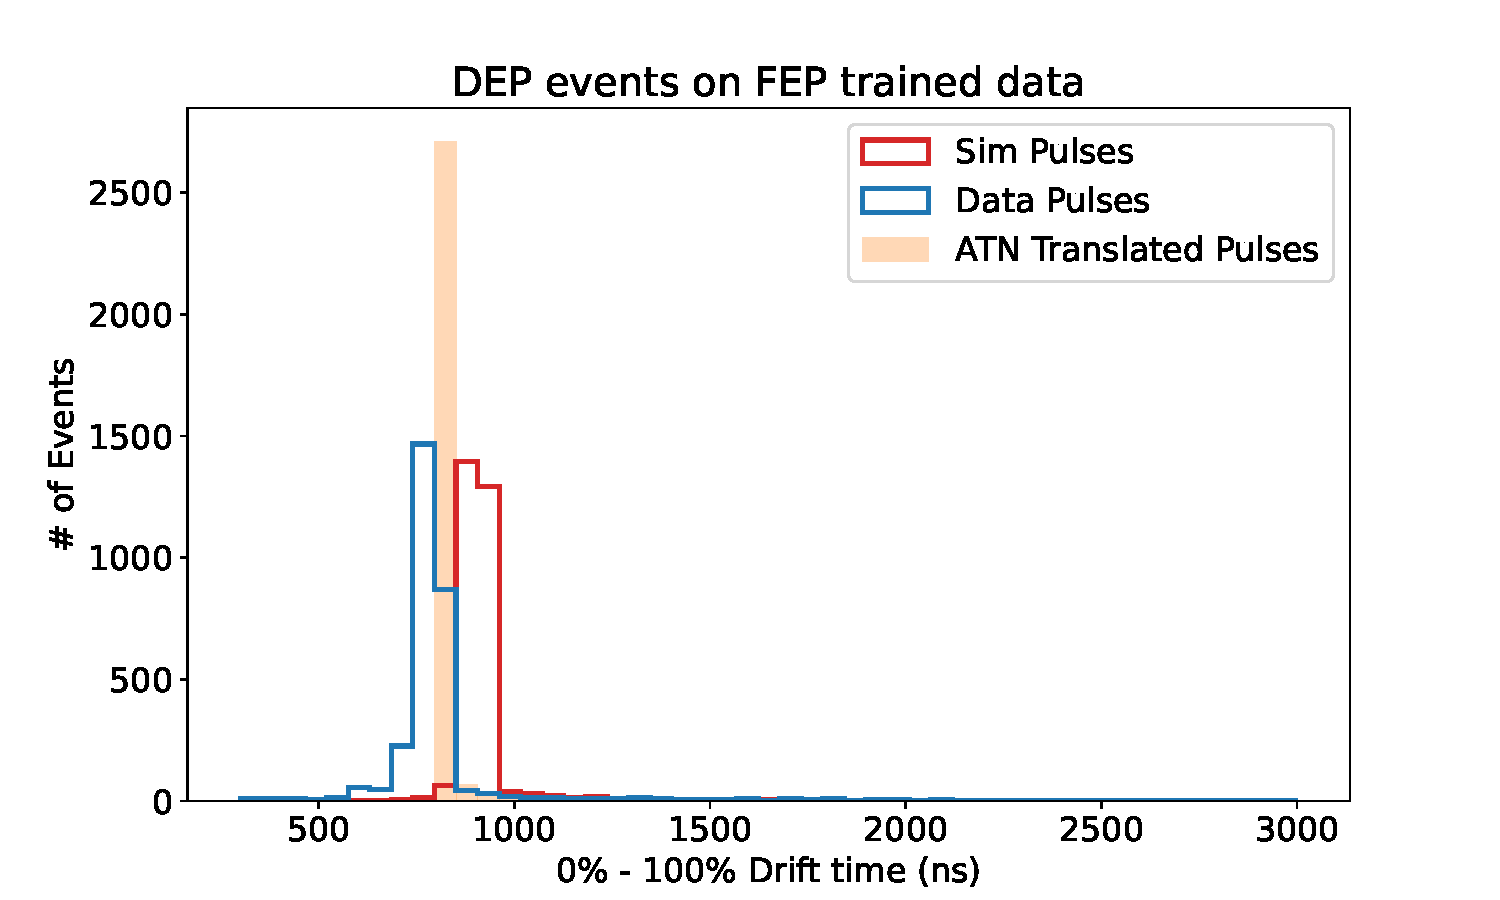
\includegraphics[width=0.95\linewidth,trim={0pc 0pc 0pc 0pc},clip]{ch8/figs/dep_drift_time.pdf}
\caption{The distribution of the 1\%–100\% drift time on DEP dataset.}
\label{fig:drift_times_dep}
\end{figure}

\subsection{Current Amplitude}

The maximum current amplitude ($I_{max}$) is determined by differentiating the waveform and identifying the maximum value of its derivative. For a given event energy, single-site events produce a localized energy deposition, resulting in a sharper and faster increase in $I_{max}$. In contrast, multisite events, characterized by energy deposition at multiple locations within the detector, yield broader and more gradual current peaks. This distinction makes $I_{max}$ highly effective in differentiating single-site from multi-site events, thereby establishing it as a crucial parameter in waveform shape simulations \cite{mjd_psd}. 

The method for calculating the current amplitude is as follows. 
\begin{figure}[!htb]
    \centering
    %[trim={left bottom right top},clip]
    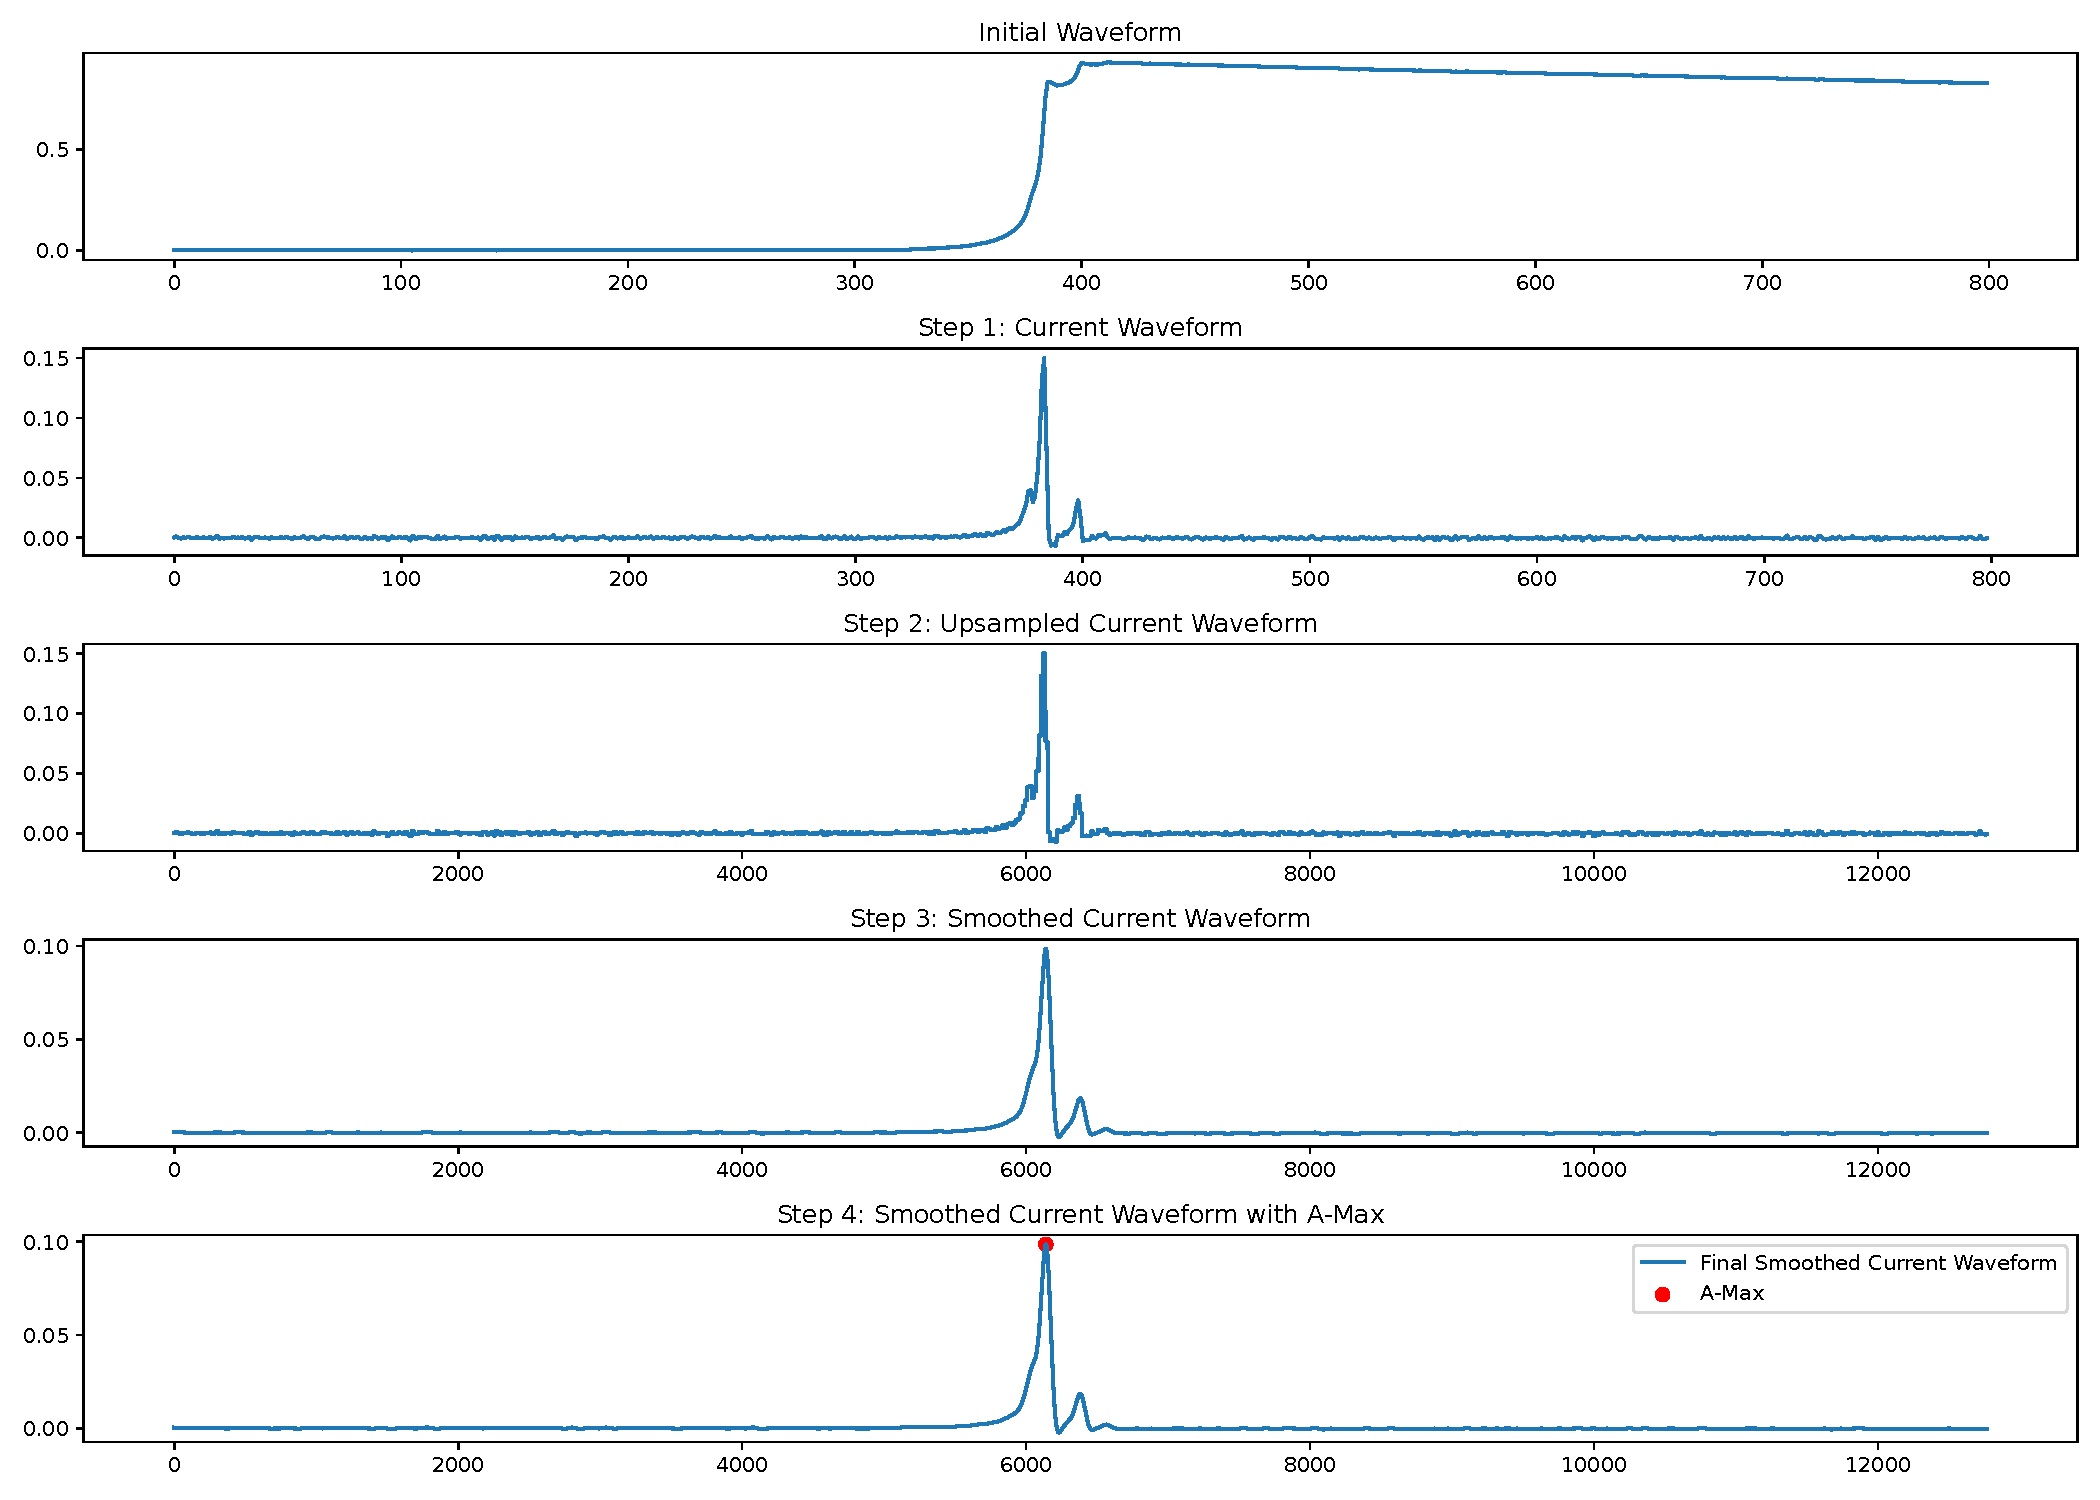
\includegraphics[width=0.99\linewidth, trim={0pc 1pc 0pc 0pc},clip]{ch8/figs/curr_amp_calc.pdf}
    \caption{Steps involved in calculating the maximum current amplitude of the waveform}
    \label{fig:ch8:curr_amp_calc}
\end{figure}

Figure \ref{fig:current_amp} illustrates the distribution of $I_{max}$.  ATN learns to correctly slow the current amplitude of the simulated waveforms to align with the data. The SEP $I_{max}$ increases to IoU to $63.71\%$ from $27.53\%$.
  
\begin{figure}[htb!]
\centering
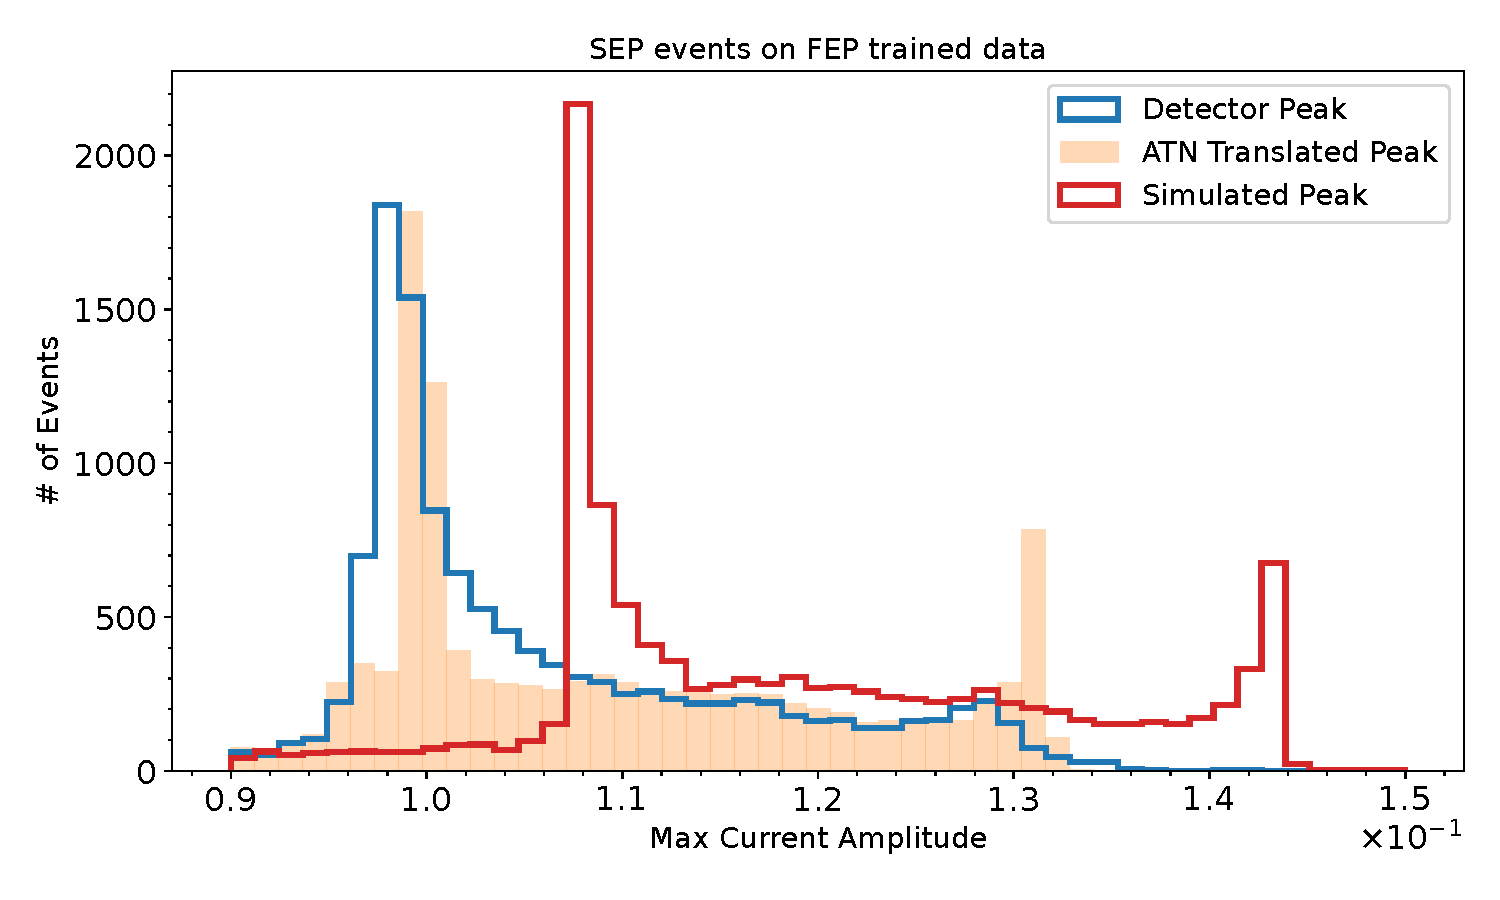
\includegraphics[width=0.99\linewidth,trim={0pc 0pc 0pc 0pc},clip]{ch8/figs/SEP_amp.pdf}
\caption{ Distribution of maximum current amplitude ($I_{max}$) on SEP validation datasets.}
\label{fig:current_amp_sep}
\end{figure}

\begin{figure}[htb!]
\centering
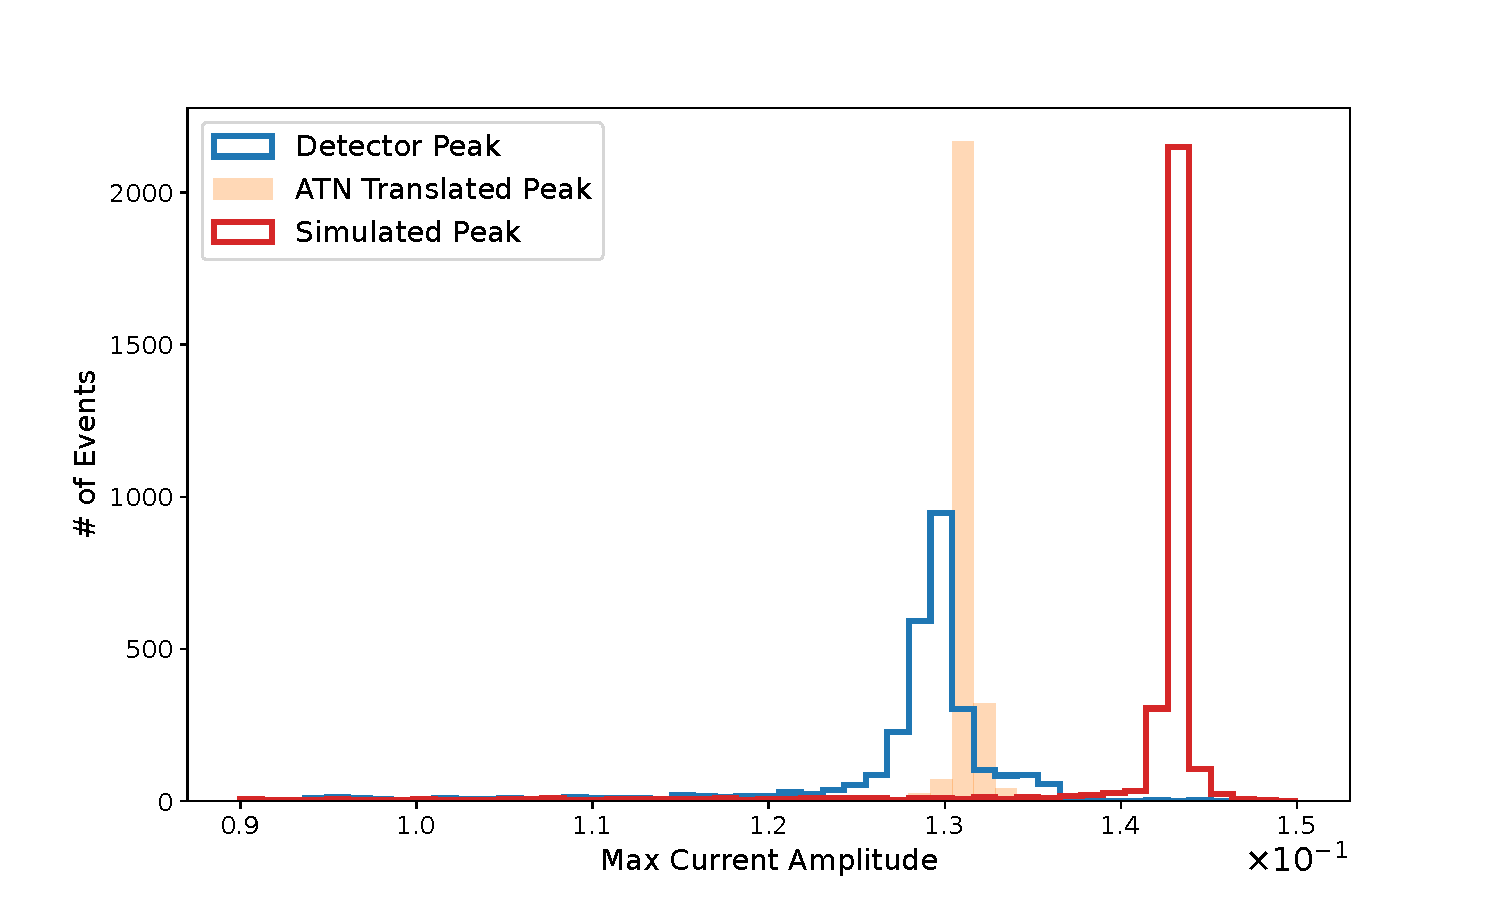
\includegraphics[width=0.99\linewidth,trim={0pc 0pc 0pc 0pc},clip]{ch8/figs/DEP_amp.pdf}
\caption{ Distribution of maximum current amplitude ($I_{max}$) on DEP validation datasets.}
\label{fig:current_amp_dep}
\end{figure}

The scatter plot between $I_{max}$ of the simulated waveforms and the translated waveforms of ATN shows that ATN performs this while maintaining the relative order of events.

\begin{figure}[htb!]
\centering
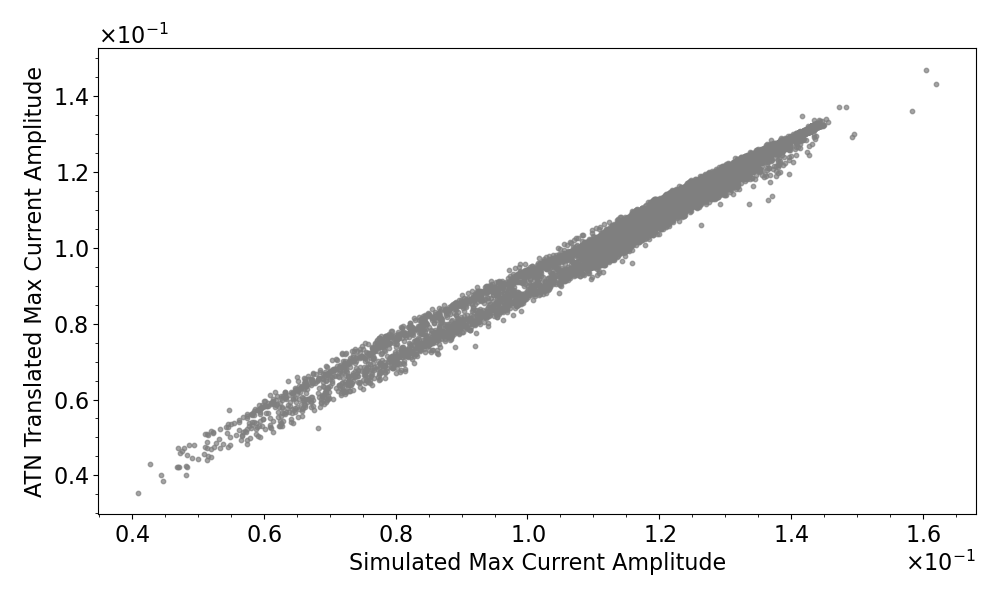
\includegraphics[width=0.99\linewidth,trim={0pc 0pc 0pc 0pc},clip]{ch8/figs/SEP_scatter_current_amplitude.png}
\caption{Scatter plot between $I_{max}$ of simulated waveforms and ATN translated waveforms. ATN shits the amplitude distribution to align with data while maintaining the relative ordering of individual events.}
\label{fig:current_amp}
\end{figure}



\subsection{Tail Slope}
The strength of the RC decay can be measured by the mean tail slope parameter $c_{tail}$. The tail slope was calculated by a linear fit of the logarithm of 300 samples of the waveform. The simulation waveforms do not have an RC decay and thus have a mean tail slope of zero; the data waveform was found to have a tail slope of $-2.946\times10^{-4}$.  Figure \ref{ch8_fig_tail_slope_comp} shows the relative magnitude of the tail slopes for simulations, data, and ATN translated waveforms. The ATN learns to match the data very well, within $0.58\%$ of the actual value.


\begin{figure}%[!htb]
\centering
%[trim={left bottom right top},clip]
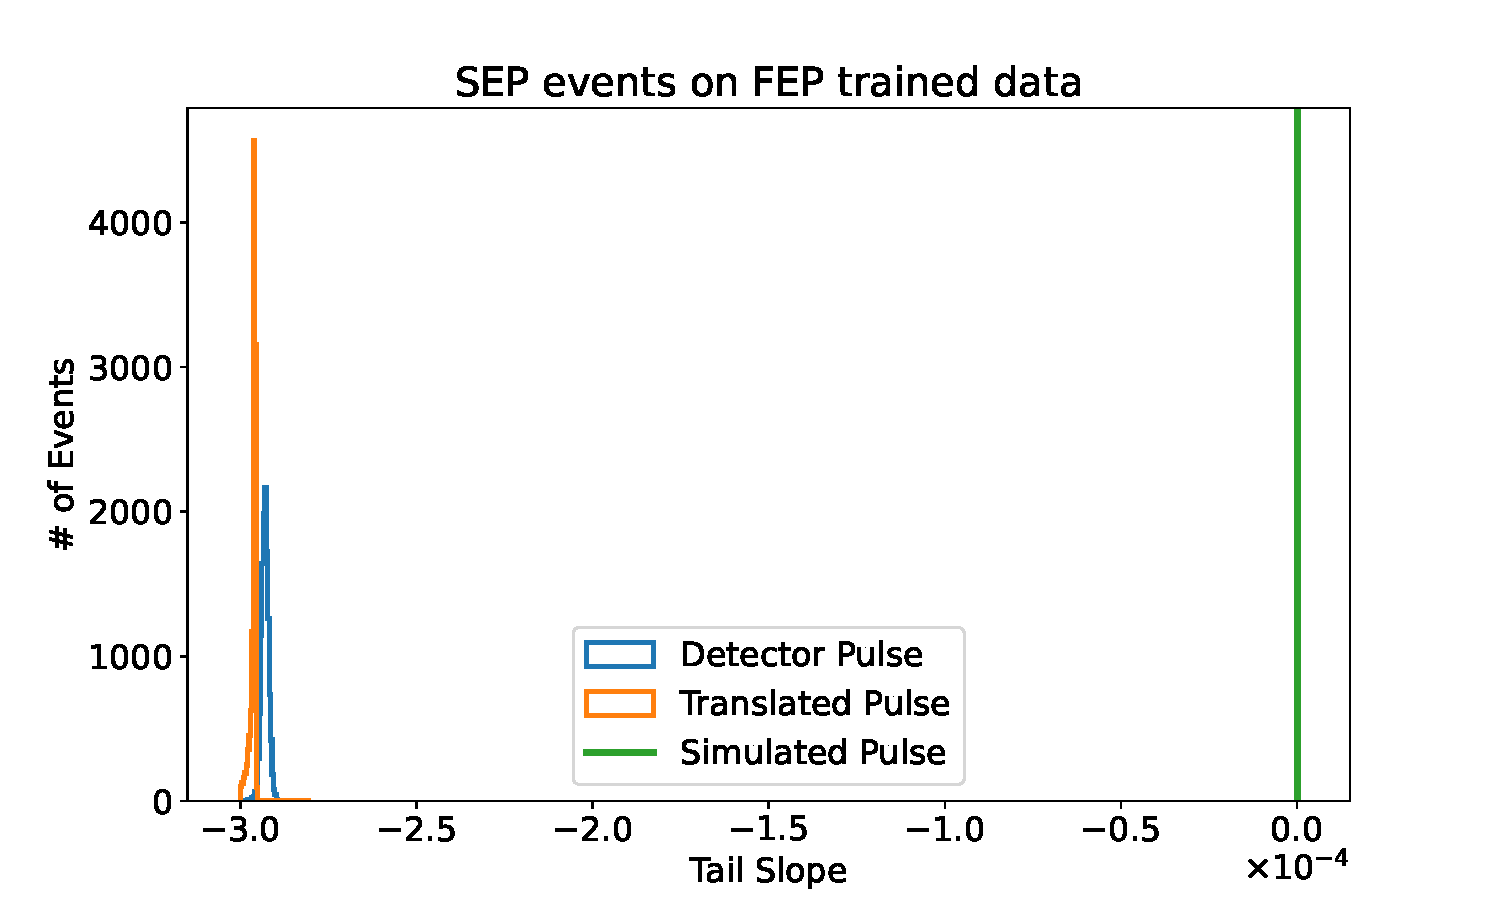
\includegraphics[width=0.97\linewidth,trim={2pc 0pc 2pc 0pc},clip]{ch8/figs/SEP_sim_ts.pdf}
\caption{Distribution of tail slope for simulations, data, and ATN translated waveforms.}
\label{ch8_fig_tail_slope_comp}
\end{figure}

Figure \ref{ch8_fig_tail_slope_sim} shows the comparison of the tail slope between the data and the ATN translated waveforms. The distributions are not identical. This could be due to numerical precision and adversarial training.

\begin{figure}%[!htb]
\centering
%[trim={left bottom right top},clip]
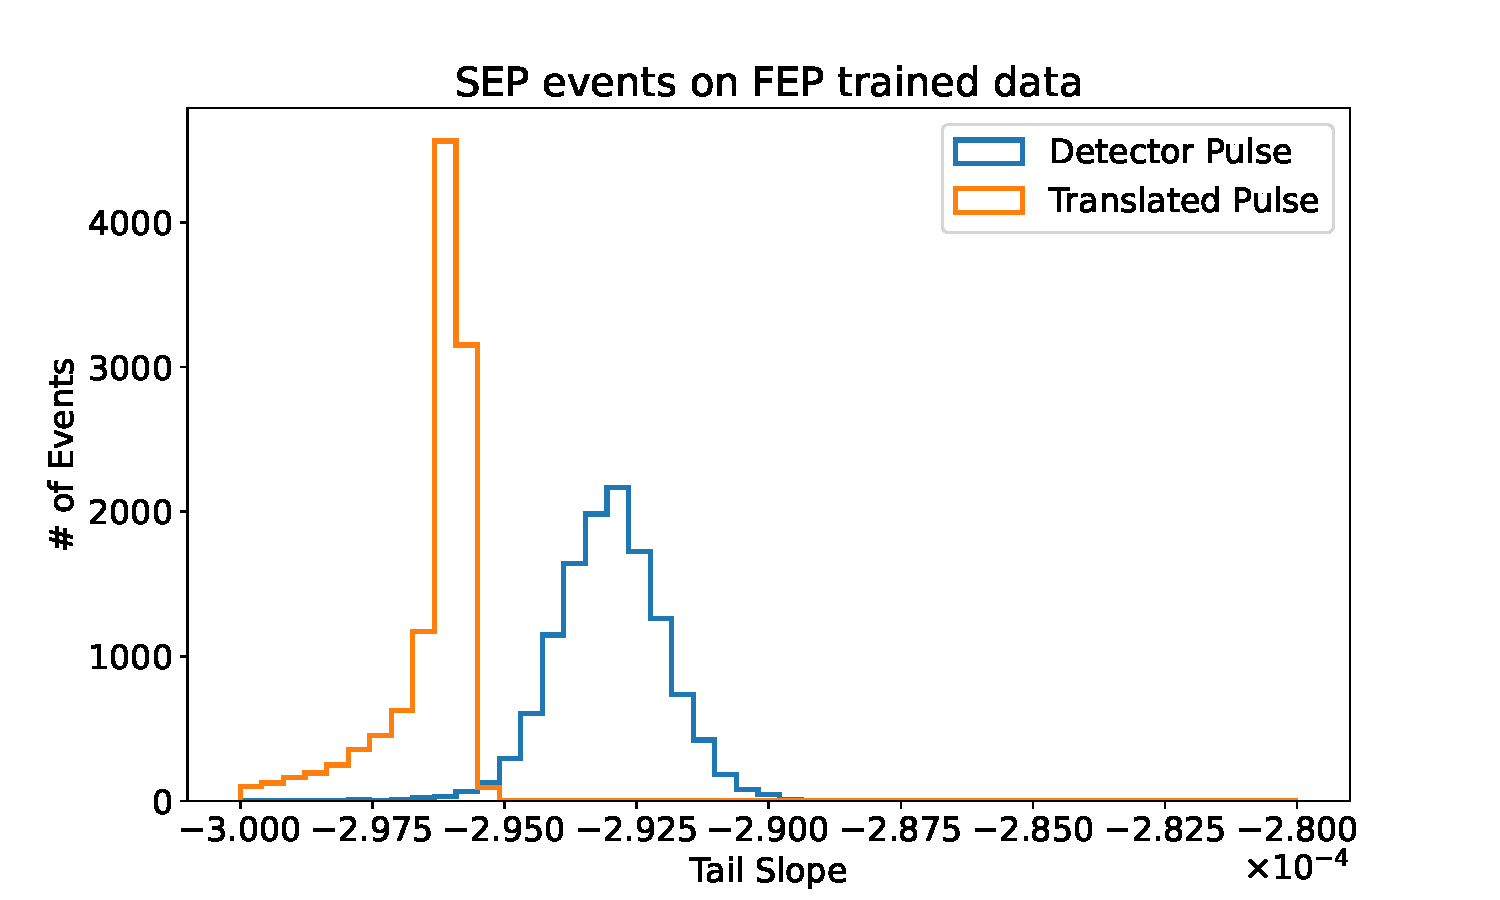
\includegraphics[width=0.9\linewidth,trim={2pc 0pc 2pc 0pc},clip]{ch8/figs/SEP_ts.pdf}
\caption{Distribution of tail slope between data and ATN translated waveforms}
\label{ch8_fig_tail_slope_sim}
\end{figure}

Although our primary focus in this paper is on translating simulations to resemble measured data, CPU-Net’s bidirectional nature also makes it a powerful tool for denoising real detector waveforms. By transforming noisy detector signals into cleaner, simulation-like waveforms, CPU-Net can help isolate and identify subtle features in the event topology. This capability could ultimately improve spatial reconstruction and improve our understanding of particle interactions within the detector.
